\chapter{Domain peering evaluation}
In this chapter, we present the analyses conducted on the logical domain grouping implementation, chosen for its higher resilience compared to the multi-level implementation.

\section{Test Environment}
The test environment was created by leveraging the functionalities of Crownlabs, an open-source platform associated with the Politecnico di Torino, which was developed during the years of the Coronavirus spread.

\subsection{Crownlabs}
Crownlabs is an open-source project created to provide students with access to laboratory systems and services during the challenging times of the coronavirus pandemic, which imposed severe travel restrictions. In fact, the name derives from the virus itself and its initial purpose, as "Crown" translates to "Corona" in Italian and labs measn laboratories.

The authors of this project were a group of volunteers primarily composed of MSc students who, within just a few weeks of very hard work, as described on the project website \cite{e1-1}, managed to deliver a functioning version, to address the university places closures mandated by the Italian government.

Nowadays, Crownlabs continues to be supported by students, and its functionalities have expanded: it not only allows the remote use of laboratory machines through a web browser, enabling both personal exercises and group work, but also leverages the Politecnico di Torino's data center to instantiate and use virtual machines transparently within an internal network.

It is precisely this latter functionality that has been utilized, as the Kubernetes clusters used were composed of these virtual machines.

\subsection{Nodes configuration}
Each virtual machine representing a node in a cluster possesses the following characteristics, chosen to simulate low computational capacity typical of devices found in energy monitoring and distribution stations.
\begin{itemize}
\item \textbf{Operating system:}  Ubuntu server 20.04 LTS.
\item \textbf{CPU:} 4 core.
\item \textbf{RAM:} 8 GB.
\item \textbf{Disk memory:} 25 GB.
\end{itemize}

\subsection{Software configuration}
Di seguito vengono specificate le versioni delle piattaforme utilizzate:
\begin{itemize}
\item \textbf{K3s:} v1.24.17+k3s1.
\item \textbf{Liqoctl:} v0.10.2.
\item \textbf{Liqo:}  v0.10.2.
\item \textbf{PDC:}  v2.4.
\item \textbf{Database:} Percona XtraDB operator v1.11.0.
\item \textbf{Database connector:} MYSQL connector v8.2.
\end{itemize}

It should be noted that certain parameters of the k3s kubelet and manager controller have been adjusted to decrease the cluster response time in case of failure, as detailed in the table \ref{t:1}.

\begin{table}[ht]              
\centering 
\begin{tabularx}{\textwidth}{|l|c|X|}
\hline 
\textbf{Option} &\textbf{Value} &\textbf{Description} \\
\hline
\raisebox{-0.25cm}{node-status-update-frequency} & \raisebox{-0.25cm}{10s -> 5s} & Specifies how often kubelet posts node status \\
\hline
\raisebox{-1.5cm}{node-monitor-grace-period} & \raisebox{-1.5cm}{40s -> 20s} & Specifies the amount of time in seconds that the Kubernetes Controller Manager waits for an update from a kubelet before marking the node unhealthy. Must be N times more than kubelet's nodeStatusUpdateFrequency, where N means number of retries allowed for kubelet to post node status \\
\hline
\raisebox{-0.5cm}{pod-eviction-timeout} & \raisebox{-0.5cm}{300s -> 5s}&This parameter specifies how long Kubernetes waits before evicting pod from a node marked as "NotReady" \\
\hline
\end{tabularx}
\caption[Kubelet and Controller Manager list of parameter changes]{Kubelet and Controller Manager list of parameter changes} \label{t:1}  
\end{table}

\subsection{Cluster configuration}
Due to the limit of 5 virtual machines, the system was organized into 5 Kubernetes clusters, each comprising a single node. As shown in Figure \ref{graph:test}, the topology is a fully-meshed star topology where the root cluster occupies the central position, hosting all deployments of the PMU, PDC, and database applications. Through Liqo peering, it offloads the test namespace to the leaf clusters.

The leaf clusters are connected by unidirectional peering for the transparent operation of the distributed Percona database system, and they will be the only locations where the pods of the aforementioned applications can be scheduled.

\begin{figure}[ht]\centering
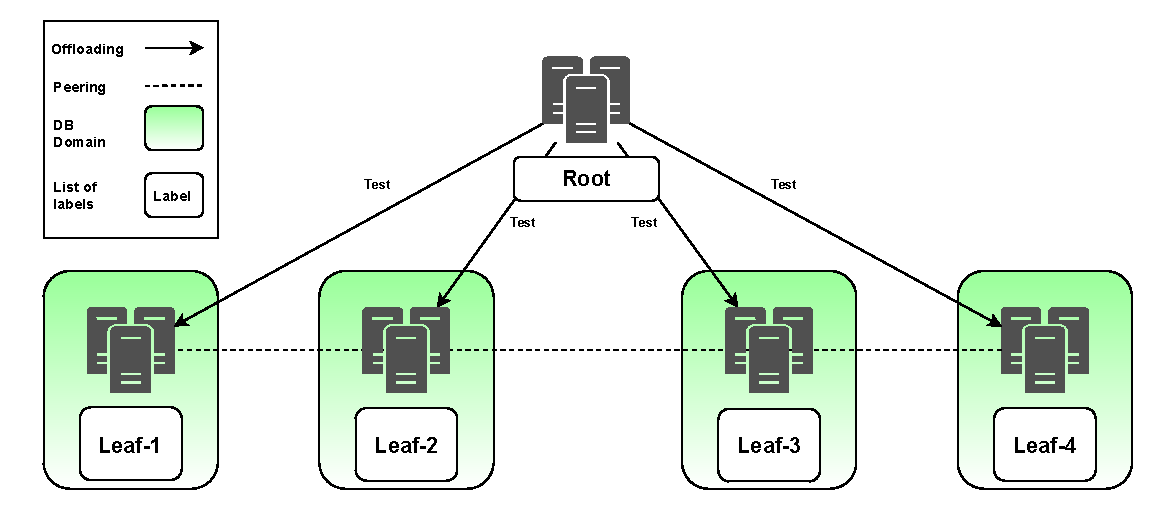
\includegraphics[scale=0.5]{Pictures/test}
\caption{Configuration test environment}\label{graph:test}
\end{figure}

\section{Latency}
In this section, we demonstrate the latency increase due to the overhead generated by Liqo technology, using 4 virtual machines, where one is consistently used as the secondary member (Root), while the others represent the primary member for each test (Leaves).

Considering that data in our architecture is transmitted using TCP protocols, which utilize acknowledgments (ACKs), latency is measured as the round-trip time of a packet. The following tests were conducted using the ping command, with approximately 1000 iterations per test, individually executed from the Leaf machines to the Root machine.

Firstly, to establish a baseline for the tests, the network latency was calculated by averaging the mean of three ping values obtained from the virtual machines towards the root machine, as shown in the table \ref{t:2}.

\begin{table}[ht]              
\centering 
\begin{tabular}{|l|c|}
\hline
\textbf{Virtual machine} & \textbf{Latency}  \\ 
\hline
Leaf-1 & 0.689 $\pm$ 0.447  \\
\hline
Leaf-2 & 0.760 $\pm$ 0.771 \\
\hline
Leaf-3 & 0.715 $\pm$ 0.468 \\
\hline
Avg & 0.721 $\pm$ 0.581 \\
\hline
\end{tabular}
\caption[Network average latency ]{Network average latency} \label{t:2}  
\end{table}

After establishing the network latency, we proceed to calculate the latency between a pod located on different Leaf nodes and a pod in the Root node, where the Leaf nodes and the Root node belong to the same cluster, shown in Table \ref{t:3}, or belong to different clusters peered with Liqo, shown in Table \ref{t:4}.

\begin{minipage}{0.45\textwidth}
  \centering
  \vspace{0.5cm}
  \begin{tabular}{|l|c|}
  \hline
  \textbf{Cluster Node} & \textbf{Latency}  \\ 
  \hline
  Leaf-1 & 0.735 $\pm$ 0.294  \\
  \hline
  Leaf-2 & 0.992 $\pm$ 0.568 \\
  \hline
  Leaf-3 & 0.936 $\pm$ 0.483 \\
  \hline
  Avg & 0.888 $\pm$ 0.267 \\
  \hline
  \end{tabular}
  \captionof{table}{Latency between pod on different nodes, but on the same cluster}
  \label{t:3}\vspace{0.5cm}
\end{minipage}%
\hspace{0.05\textwidth} % Adjust the horizontal space between the tables
\begin{minipage}{0.45\textwidth}
  \centering
  \vspace{0.5cm}
  \begin{tabular}{|l|c|}
  \hline
  \textbf{Remote Node} & \textbf{Latency}  \\ 
  \hline
  Leaf-1 & 1.269 $\pm$ 0.724  \\
  \hline
  Leaf-2 & 1.400 $\pm$ 0.829 \\
  \hline
  Leaf-3 & 1.368 $\pm$ 0.903 \\
  \hline
  Avg & 1.346 $\pm$ 0.821 \\
  \hline
  \end{tabular}
  \captionof{table}{Latency between pod on different clusters, peered with Liqo}
  \label{t:4}\vspace{0.5cm}
\end{minipage}

The increase due to Liqo is measured by subtracting the average latency from Table \ref{t:3}, which is the sum of network latency + Kubernetes overhead, from the average latency shown in Table \ref{t:4}, which is the sum of network latency + Kubernetes overhead + Liqo overhead. This calculation yields the result shown in Table \ref{t:5}.

\begin{table}[ht]              
\centering 
\begin{tabular}{|l|}
\hline
\textbf{Average Liqo Latency} \\ 
\hline
0.458 ± 0.864 ms \\
\hline
\end{tabular}
\caption{Average Liqo Latency} \label{t:5}  
\end{table}

The latency between pods on different Kubernetes clusters without multi-cluster technologies was not tested, as the goal is to demonstrate the latency increase using Liqo across different clusters compared to using a single Kubernetes cluster connecting all nodes.

\section{k3s reaction time}

In the upcoming test, two clusters of virtual machines connected via unidirectional Liqo peering were utilized: the consumer cluster and the provider cluster. The objective was to show the consumer cluster's response time in the event of disconnection of the virtual node representing the provider cluster, for any reason.

The test involved two scripts. The first script disabled the network interface on the virtual machine running Liqo in the provider cluster and recorded the timestamp. The second script executed a loop on the consumer cluster, running 'kubectl get node' every 0.4 seconds, and appending the output with a timestamp. (A shorter interval wasn't feasible due to the command execution time.)

The results are depicted in graph A. \ref{graph:k-reaction}.

\begin{figure}[!htb]\centering
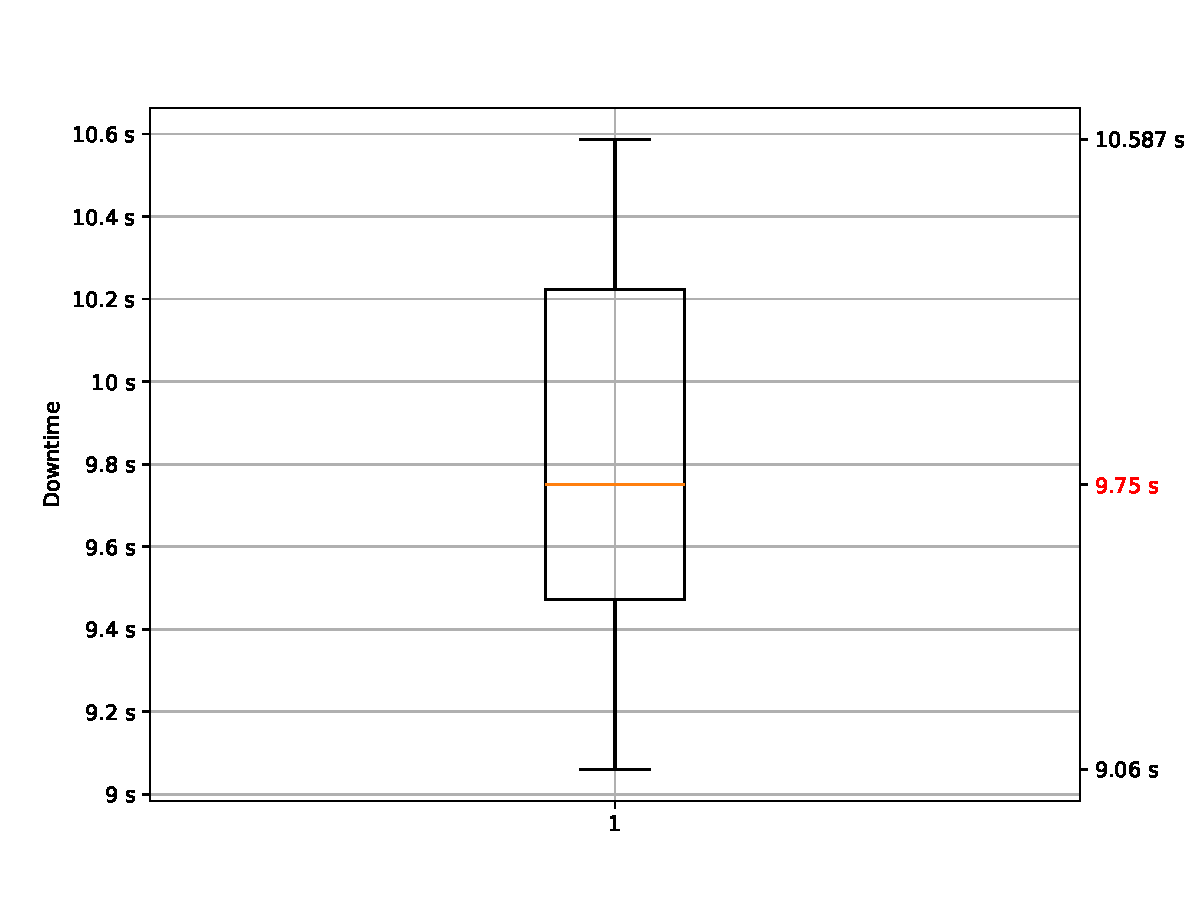
\includegraphics[scale=0.5]{Pictures/k3s-reaction}
\caption{Reaction to set virtual node as Not Ready in case of remote cluster disconnession}\label{graph:k-reaction}
\end{figure}

\section{Stream reaction time}
The following tests demonstrate the downtime of a data stream from a PMU in the following scenarios:

\begin{enumerate}
\item Internal failure of a PDC pod, resulting in the rescheduling of the application. 
\item Fault/disconnection of the cluster hosting a PDC pod, resulting in the application being rescheduled to another cluster.
\end{enumerate}

Downtime is calculated from the timestamp of the last data frame of the old stream to the timestamp of the first data frame of the new stream, encompassing the time required for rescheduling the PDC pod, retrieving configurations from the database system, and reconnecting to the data stream.

These tests examine a data stream originating from a PMU that traverses through two PDC pod, one considered low-level and the other considered high-level, before reaching its intended application.

The use of the data frame timestamp is crucial due to the PMU's real-time production of data frames at 33-millisecond intervals, ensuring precise downtime calculations and analysis.
\subsection{Pod failure}
The failure scenario of the PDC pod was simulated by customizing the liveness probe mechanism, intentionally triggering a failure check after the pod had been running for 60 seconds.

The test results, displayed in graph \ref{graph:pod-down}, illustrate the median duration required for the lower-level PDC application to resume normal operation. This duration encompasses the time from detecting the PDC pod failure to its subsequent recovery, including the processes of restarting the pod, retrieving configurations from the system database, and re-establishing connection to the data stream.

\begin{figure}[ht]\centering
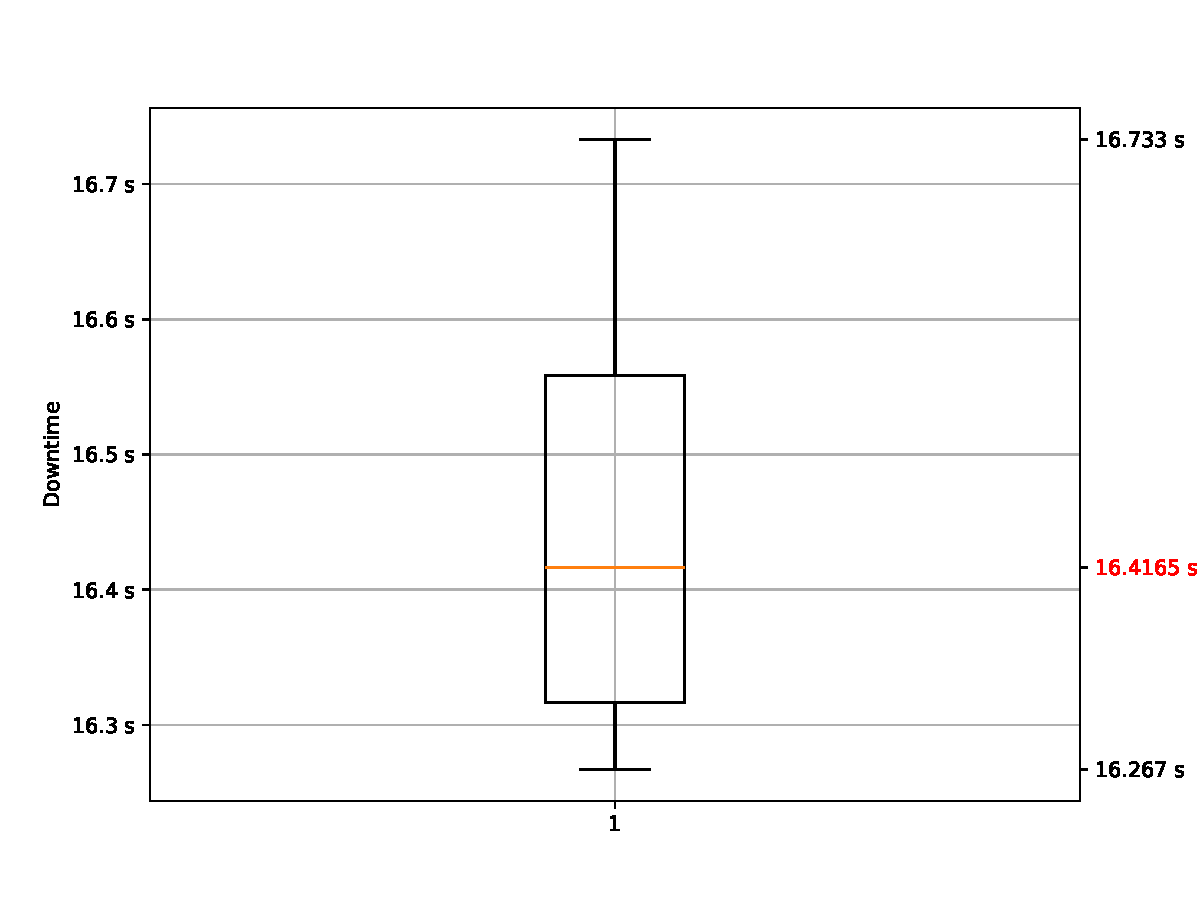
\includegraphics[scale=0.5]{Pictures/pdc-pod-down}
\caption{Box plot regarding stream downtime from last old data to the first new data in case of pod failure}\label{graph:pod-down}
\end{figure}

\subsection{Cluster failure}
The failure scenario of the cluster containing the lower-level PDC pod was simulated by directly disabling its network interface.

The test results, displayed in graph \ref{graph:cluster-down}, illustrate the median duration required for the lower-level PDC application to resume normal operation. This duration includes the time required for the cluster to detect that the virtual node hosting the PDC is unreachable (9.75 seconds as shown in graph \ref{graph:k-reaction}), the waiting time before it can be rescheduled to another node (5 seconds as indicated in table \ref{t:1}), and the time necessary for the pod to restart (16.41 seconds as depicted in graph \ref{graph:pod-down}).

\begin{figure}[ht]\centering
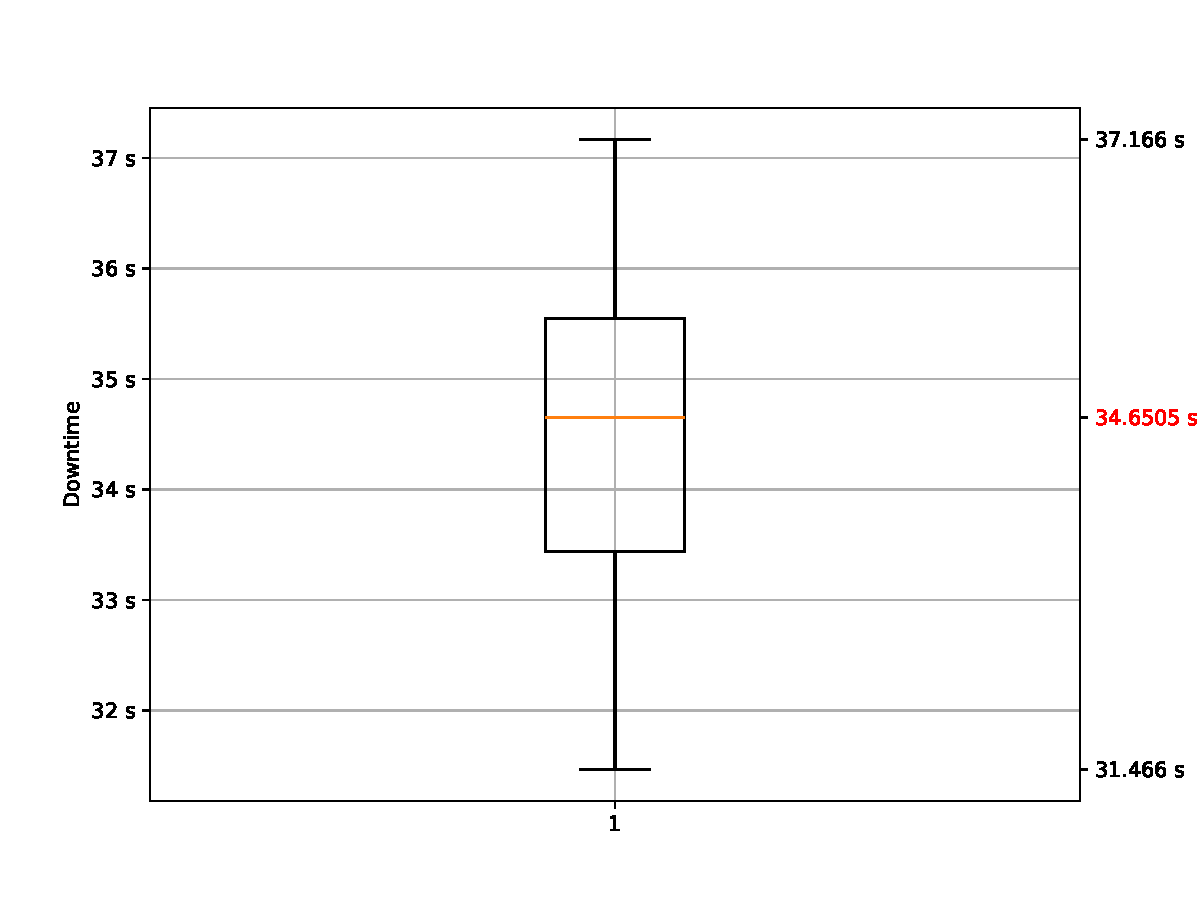
\includegraphics[scale=0.5]{Pictures/pdc-cluster-down}
\caption{Box plot regarding stream downtime from last old data to the first new data in case of cluster failure}\label{graph:cluster-down}
\end{figure}



